\documentclass[11pt,twocolumn]{report}
\usepackage{graphicx}
\usepackage{a4wide}
\usepackage[english]{babel}
\usepackage{amsfonts}
\usepackage{amsthm}
\usepackage{amsmath}
\graphicspath{ {images/} }

\author{He Chen, Henri Maxime Demoulin, Gabrielle De Micheli}
\title{CIS520 Final Project Report}

\begin{document}
\maketitle
\section*{Methods Accuracy Report}
    % Results for each method you tried (try to use checkpoints to get test set accuracy for each of your methods)
	First, let us mention that when we write training error, we refer to our training error after cross-validation. When we write test error, we refer to the leaderboard.\\
    
    Firstly, let us explain some preprocessing ideas for the words. We start by deleting all the English, French and Spanish stop words and the words containing only one character (usually ponctuation). We also delete all the words that start with $\backslash u$. This corresponds to unicode. Finally, we try to remove the http and rt (note that we have a slightly smaller accuracy when we add the French and Spanish stop words and deleted the http and rt).  Another preprocessing idea was to iterate the words to appear only once in the entire dataset. However, this method wasn't very conclusive. The final error is $0.0967$.
    
    \subsection*{Generative Methods}
    \subsubsection{Naive Bayes}
    We start by using Naive Bayes only on the words. This method gave us around $80 \%$ of test-accuracy on the words without preprocessing. If we do the preprocessing described above, the accuracy rises to $81.42\%$. In order for Naive Bayes to work, we got rid of all the words that do not appear in any tweets because Naive Bayes assumes conditional independence. In order to use a variation of the bag of word model, the words are set to 1 if they appear in a tweet and zero otherwise. We also test Naive Bayes with all four datasets using the bag of words model.  
   
   
    
    \subsection*{Discriminative Methods}
    \subsubsection{Linear Regression}
    
    
     \subsubsection{Random Forest}
     "We tried random forest only on the words but we observed the following: with 20 trees, we had a training error of 0.2167 and with 100 trees a training error of 0.2116. We use the same preprocessing process that with Naive Bayes".(DELETE MAYBE)\\
     For 100 trees, the error is 0.0533. For 500 trees, we get 0.0520 and for 1000 trees, we get 0.0509. For the last case, the accuracy is of 0.7776.
    \subsubsection{SVM}
    
    If we use SVM with an RBF (Radial Basis Function) kernel function, we have a training error of 0.3813. Without RBF, the training error is 0.26. The linear kernel is twice as accurate as the RBF function. However, if we use RBF but this time without the word-count, we have a training error of 0.3776, which is greater than the error obtained with the two previous combinations we tried. If we try to use SVM without the word-count and without RBF, the training error is 0.2626. We also try SVM only on words, and notice that it performs better than KNN.
    
    \subsubsection*{Perceptron}
    TO DO
    \subsection*{Instance based Methods}
    \subsubsection{KNN}
    
    We use KNN on all four datasets and get a traning error (cross-validation) of 0.3556.
   
    \subsection*{Regularization Method}
    our own regularization method other that the standard $L_i$ penalty....
    TO DO
    \subsection*{Semi-supervised dimensionality reduction}
    \subsubsection*{PCA}
    We try using PCA on the \textit{image dataset}. First, we use PCA with all the PCs combined with SVM which gives a training error of 0.0324. We do the same again but only with 1000 PCs. This gives an error of 0.1198. Moreover, using 570 PCs (corresponding to 50MB), we get a training error of 0.1509.\\
    
    
   On the \textit{word dataset}, we also try using PCA with various numbers of PCs (all, 500 ...) and this time, combined with random forest. This gives a training error of 0.0064. The test-accuracy is 0.7491.\\
    
    

\section *{Methods Analysis}
    % Analysis of your experiments. What worked and what didn’t work? Why not? What did you do to try to fix it? Simply saying “I tried XX and it didn’t work” is not enough.
TO DO
\section*{Visualization}
    % An interesting visualization of one of your models. For instance, find the words that most correlate with the outcome. 
    We consider the well-classified words and we want to find which words are the most important. In order to visualize this, we compute a word cloud. 
    
    \begin{center}
    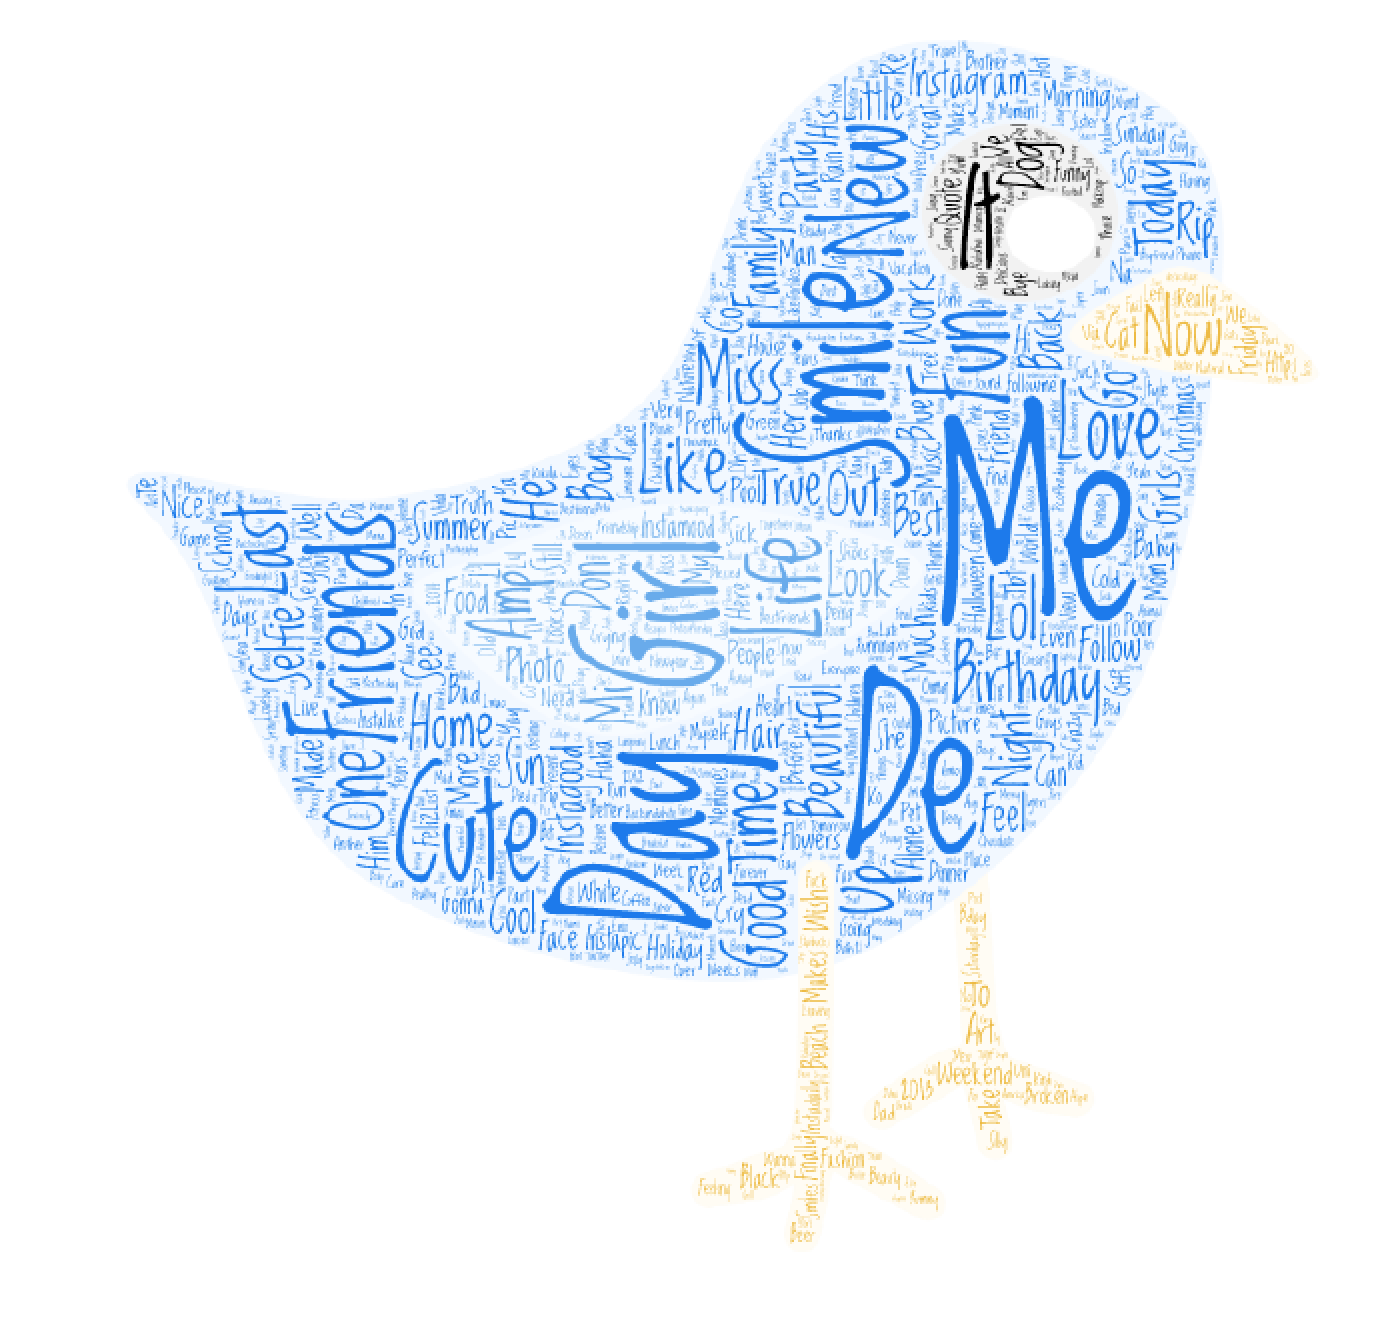
\includegraphics[scale=0.3]{cloud}
    \end{center}
    

\end{document}

